
The \SCARVSOC is split into two layers:
1) A ``inner" layer, which contains the CPU, local memories, local
   interconnect and any in-house peripherals.
2) A ``outer" layer, which wraps the ``inner" layer with vendor specific
   peripherals.
This separation allows vendor IP and peripherals to be gradually brought
into the inner layer as open-source or in-house alternatives are
found or developed.
Figure \ref{fig:design:soc-blocks} shows the \SCARVSOC block diagram.

\begin{figure}
\centering
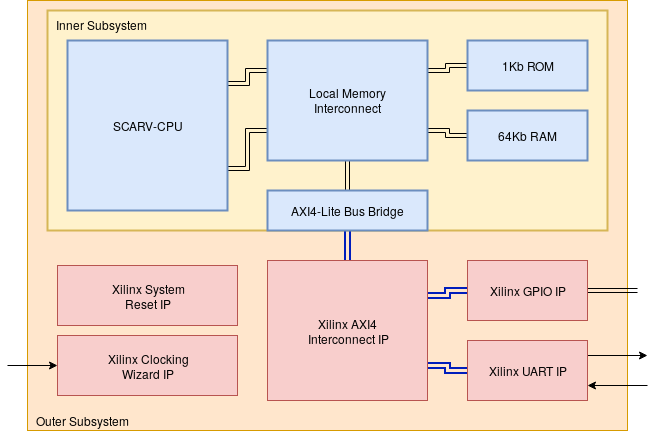
\includegraphics[width=0.8\textwidth]{image/soc-block-diagram.png}
\caption{
Block diagram of the \SCARVSOC, showing the inner subsystem which can be
implemented anywhere, and the Xilinx-specific outer subsystem.
}
\label{fig:design:soc-blocks}
\end{figure}

\noindent The principle components of the inner layer are:

\begin{enumerate}
\item The SCARV-CPU.
\item The local memory interconnect.
\item The local RAM and ROM memories.
\item An AXI4-Lite bus bridge, which connects the core subsystem to
      external peripherals.
\end{enumerate}


\noindent The current Xilinx specific outer layer is made up of:

\begin{enumerate}
\item System clock generation.
\item System reset control.
\item AXI UART peripheral.
\item AXI GPIO peripheral.
\end{enumerate}

